
% ----------------------------------------------------------------------
\subsection{ Módulo de generación de señales}

% C- Módulo de generación de medidas asociadas a una trayectoria
% - Objetivo del módulo		
En este módulo se podrán simular distintos tipos de señales a partir de la trayectoria generada. El objetivo es generar datos que los algoritmos de localización procesarán. Al igual que en el módulo anterior, los modelos de simulación son cruciales para que el comportamiento del simulador sea fiel a la realidad. 

% - Modelización	
%     - Tipos de señales y métricas			
En Navindoor se ha creado la clase abstracta \emph{Signal} con propiedades que contiene la información de las medidas a lo largo de un periodo de tiempo. Además, se ha creado dos clases que heredan los métodos y propiedades de la clase \emph{Signal}. Estas son:
\begin{itemize}
    \item La clase \emph{BeaconBased}: Representando señales que necesitan  puntos de acceso para poder ser simuladas. 
    \item La clase \emph{BeaconFree}: Representando señales que pueden ser simuladas sin la necesidad de los puntos de acceso.
   \end{itemize}

Dentro del entorno de simulación, las diferencias entre estas clases se ven en la forma de construirlas. Mientras que la clase \emph{BeaconFree}, solo necesita la información de la trayectoria para ser definida, la clase \emph{BeaconBased} necesita los objetos \emph{beacons} definido en el módulo de la planimetría (figura \ref{schemaBB}). 

La clase \emph{BeaconBased} puede representar señales de atenuación de nivel de potencia (RSS), ángulo de llegada (AoA) y tiempo de vuelo (ToF), mientras que la clase \emph{BeaconFree} puede representar señales inerciales (aceleraciones lineales y velocidades angulares), intensidades de campo magnético y presión atmosférica. Los modelos de simulación de señales utilizados por defecto son básicos con una componente de ruido gaussiano.

% \begin{table}[ht]
%     \centering
%     \begin{tabular}{|c|c|}
%         \hline
%         {\textbf{BeaconBased}} & {\textbf{BeaconFree}}          \\ \hline
%         {Atenuación de nivel de potencia (RSS)}    & Barómetro        \\ \hline
%         {Tiempo de vuelo (ToF)}              & Acelerómetro               \\ \hline
%         {Angulo de llegada (AoA)}            & Magnetómetro             \\ \hline
%                                             & giroscopio             \\ \hline

%     \end{tabular}
%     \caption{Tipo de modelos de simulación de señales}
%     \label{tiposenales}
% \end{table}


En Navindoor se trata a los modelos como parámetros de entrada, por lo que es posible cambiarlos por modelos más complejos simplemente creando funciones con una interfaz de entrada/salida específica. En el caso de las clases \emph{BeaconBased}, los parámetros de entrada deberán ser un punto de la trayectoria y un objeto \emph{beacon}; y dar como parámetro de salida el valor de la señal. Mientras que en el caso de la clase \emph{BeaconFree}, solo se usa un punto de la trayectoria como parámetro de entrada y el valor de la señal como parámetro de salida.

%     - Diagrama de clases
\begin{figure}[ht!]
    \centering
        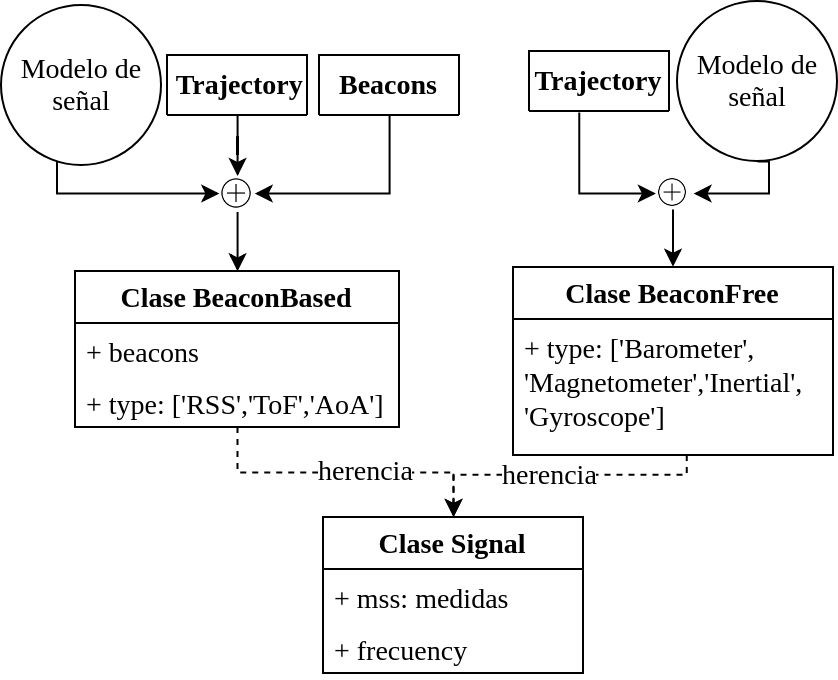
\includegraphics[width=0.85\columnwidth]{img/Design/signaldiagram.png}
        \caption{Representación de la generación de las señales.}
        \footnotesize
        Se muestra un esquema de la generación de las señales \emph{BeaconFree} y \emph{BeaconBased}. Además, también se muestra la clase \emph{Signal} de la cual heredan las propiedades donde estarán las medidas.
        \label{schemaBB}
    \end{figure} 

 

% - Explicación básica del proceso de generación de medidas asociada a una trayectoria: 
%     - Modelos de ruido: parámetros, crear modelos nuevos
%     - Visualizar señal generada
Por la parte de la GUI, en Navindoor se ha implementado un apartado para la generación de señales. En esta se muestra un listado de trayectorias previamente generadas. También se muestra un selector donde poder elegir el tipo de señal que queramos generar. Para cada uno de estos tipos nos enseña un listado de los modelos existentes. Además nos permite crear nuevos modelos a partir de una plantilla para cada tipo de señal. De esta manera dentro de la GUI podemos crear varias señales rápidamente, además de visualizar el resultado obtenido. 

% \begin{figure}[ht!]
%     \centering
%         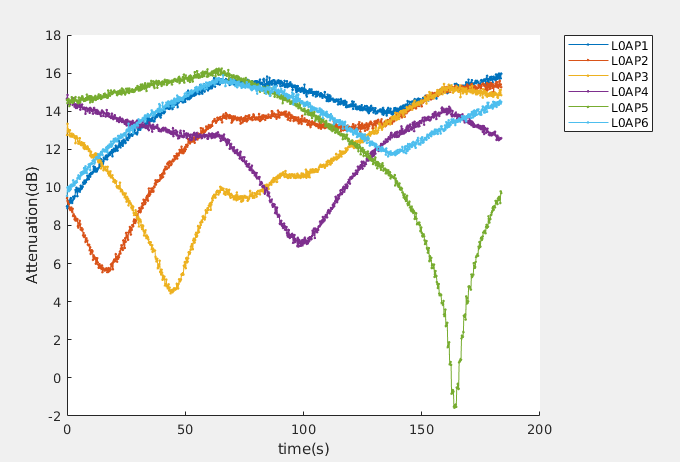
\includegraphics[width=1.0\columnwidth]{img/Design/GUIsignal.png}
%         \caption{Visualización de una señal generada en navindoor}
%         \footnotesize
%         \label{graphsBB}
%     \end{figure}
